\documentclass[12pt]{article}
\title{Supporting Information for ``Addressing Confounding and Exposure Measurement Error Using Conditional Score Functions'' by Bryan S. Blette, Peter B. Gilbert, and Michael G. Hudgens}
\date{}

\usepackage{amsmath}
\usepackage{bm}
\usepackage{caption}
\usepackage[margin=1in]{geometry}
\usepackage{natbib}
\usepackage{setspace}
\doublespacing
\allowdisplaybreaks

% Table commands to match Biostatistics journal format
\newcounter{tblcap}
%\renewcommand\thetblcap{\@arabic\c@tblcap}

\newsavebox{\tabbox}
\newsavebox{\tabnotesbox}
\newlength{\tablen}
\newlength{\tabnoteslen}
%\newcommand\centerlast{%
  %\advance\leftskip by 0pt plus 1fil%
  %\advance\rightskip by 0pt plus -1fil%
   %\parfillskip0pt plus 2fil\relax}

\long\def\tblcaption#1#2{\vspace*{-5pt}
\sbox{\tabbox}{#2}
\settowidth{\tablen}{\usebox{\tabbox}}
\vskip8pt\refstepcounter{tblcap}
\centering\parbox[c]{\textwidth}{
\centerlast\noindent\mbox{\noindent\centerlast
 Web Table \thetblcap.}\hskip4.5pt  {\it #1}}\\[7.75pt]
\fontsize{12}{13}\selectfont \mbox{#2}}

\long\def\tblcaptionnotes#1#2#3{
\sbox{\tabbox}{#2}
\sbox{\tabnotesbox}{\fontsize{9}{11}\selectfont #2}
\settowidth{\tablen}{\usebox{\tabbox}}
\settowidth{\tabnoteslen}{\usebox{\tabnotesbox}}
\vskip8pt\refstepcounter{tblcap}
\centering\parbox[c]{\textwidth}{
\centerlast\noindent\mbox{\noindent\centerlast
 Web Table \thetblcap.}\hskip4.5pt  {\it #1}}\\[7.75pt]
\fontsize{12}{13}\selectfont \mbox{#2}\\[5pt]
\parbox[@{}l]{\tabnoteslen}{\fontsize{8}{10}\selectfont #3}
}

\long\def\lantblcaption#1#2{
\sbox{\tabbox}{#2}
\settowidth{\tablen}{\usebox{\tabbox}}
\vskip8pt\refstepcounter{tblcap}
\centering\parbox[c]{48pc}{
\centerlast{\noindent\mbox{\noindent\centerlast
 Table \thetblcap.}\hskip4.5pt  {\it #1}}}\\[7.75pt]
\fontsize{12}{13}\selectfont \mbox{#2}}

\long\def\lantblcaptionnotes#1#2#3{
\sbox{\tabbox}{#2}
\sbox{\tabnotesbox}{\fontsize{9}{11}\selectfont #2}
\settowidth{\tablen}{\usebox{\tabbox}}
\settowidth{\tabnoteslen}{\usebox{\tabnotesbox}}
\addtolength{\tabnoteslen}{-2.5pt}
\vskip8pt\refstepcounter{tblcap}
\centering\parbox[c]{48pc}{
\centerlast\noindent\mbox{\noindent\centerlast
 Table \thetblcap.}\hskip4.5pt  {\it #1}}\\[7.75pt]
\fontsize{12}{13}\selectfont \mbox{#2}\\[5pt]
\hspace*{4pt}\parbox[@{}l]{\tabnoteslen}{\fontsize{8}{10}\selectfont #3}
}

\def\tblhead#1{\hline\\[-9pt]#1\\\hline\\[-9.75pt]}
\def\lastline{\\\hline}

\renewcommand{\figurename}{Web Figure}
\renewcommand{\thesection}{\Alph{section}}

\usepackage{Sweave}
\begin{document}
\Sconcordance{concordance:Web-appendix.tex:Web-appendix.rnw:%
1 75 1 1 0 222 1}


\maketitle

\section{Large Sample Properties}

In Web Appendix A, the large sample properties of the proposed estimators discussed in Section 3 of the main paper are proven.

\subsection{G-formula CSM estimator}

\subsubsection{Large sample properties}

Consistency and asymptotic normality of the g-formula estimator are proven using standard estimating equation theory~\citep{stefanski2002}. The original CSM estimator is an M-estimator and the g-formula can be written as a solution to an unbiased estimating equation. Thus, the proposed g-formula CSM estimator is an M-estimator with the estimating equation vector given in equation (3).

The parameter of interest $\text{E} \{ Y(\bm{a}) \}$ appears in the last estimating equation of (3), and the proof of consistency and asymptotic normality of the g-formula CSM estimator relies on (i) the usual g-formula proof based on the causal assumptions made in Section 2 of the main paper and (ii) that the CSM estimating equations were previously shown to be unbiased~\citep{carroll2006}. In particular, (ii) implies that $\text{E}[g^{-1}(\beta_{0} + \bm{a}\beta_{a} + \bm{L}\beta_{l} + \bm{a}\beta_{al}\bm{L}^{T}) \}] = \text{E} \{ \text{E}(Y | \bm{A} = \bm{a}, \bm{L}) \}$ and then from (i) it follows that $\text{E} \{ \text{E}(Y | \bm{A} = \bm{a}, \bm{L}) \} = \text{E}[\text{E} \{ Y(\bm{a}) | \bm{L} \}] = \text{E} \{ Y(\bm{a}) \}$.

Therefore the estimating function for the parameter $\text{E} \{ Y(\bm{a}) \}$ is unbiased. Denote $\hat{\Theta}_{GF}$ as the solution to $\sum_{i=1}^{n} \psi_{GF-CSM}(Y_{i}, \bm{L}_{i}, \bm{A}^{*}_{i}, \Sigma_{me}, \hat{\Theta}_{GF}) = 0$. Then under certain regularity conditions $\sqrt{n}(\hat{\Theta}_{GF} - \Theta_{GF}) \rightarrow_{d} N(\textbf{0}, A^{-1}B(A^{-1})^{T})$ where $A$ and $B$ are consistently estimated by

\begin{equation*}
\hat{A} = \frac{1}{n} \sum_{i=1}^{n} \frac{d}{d\Theta_{GF}^{T}} \psi_{GF-CSM}(Y_{i}, \bm{L}_{i}, \bm{A}^{*}_{i}, \Sigma_{me}, \hat{\Theta}_{GF})
\end{equation*}
\begin{equation*}
\hat{B} = \frac{1}{n} \sum_{i=1}^{n} \psi_{GF-CSM}(Y_{i}, \bm{L}_{i}, \bm{A}^{*}_{i}, \Sigma_{me}, \hat{\Theta}_{GF}) \psi^{T}_{GF-CSM}(Y_{i}, \bm{L}_{i}, \bm{A}^{*}_{i}, \Sigma_{me}, \hat{\Theta}_{GF})
\end{equation*}

\subsubsection{Relationship to classical causal estimators}

The CSM estimating equations reduce to the score equations for a generalized linear model (GLM) when the measurement error covariance matrix $\Sigma_{me} = 0_{m \times m}$~\citep{carroll2006}. Thus under no measurement error, the procedure described above reduces to solving a stack of estimating equations corresponding to the common practice of using the g-formula while specifying a GLM for the outcome regression, making this standard procedure a special case of the proposed estimator.

\subsection{IPW CSM estimator}

\subsubsection{Large sample properties}

To show $\text{E} \bigg[\frac{f(\bm{A}^{*})}{f_{0}(\bm{A}^{*} | \bm{L})} \{ Y - \text{E}(Y | \bm{\Delta})\} \bigg] = 0$, we will show that $\text{E} \bigg( \frac{f(\bm{A}^{*})}{f_{0}(\bm{A}^{*} | \bm{L})} Y \bigg) = \text{E} \left \{ \frac{f(\bm{A}^{*})}{f_{0}(\bm{A}^{*} | \bm{L})} \text{E}(Y | \bm{\Delta}) \right \}$.

First,
\begin{align*}
\text{E} \bigg( \frac{f(\bm{A}^{*})}{f_{0}(\bm{A}^{*} | \bm{L})} Y \bigg) &= \text{E} \left \{ \text{E} \middle( \frac{f(\bm{A}^{*})}{f_{0}(\bm{A}^{*} | \bm{L})} Y | L \middle) \right \} \\
&= \text{E} \left \{ \int_{a^{*}} \frac{f(\bm{a}^{*})}{f_{0}(\bm{a}^{*} | \bm{L})}  \text{E} \middle( Y | \bm{A}^{*} = \bm{a}^{*},  L \middle) f_{0}(\bm{a}^{*} | L) d\bm{a}^{*} \right \} \\
&= \text{E} \left [ \int_{a^{*}} \text{E} \middle\{ \text{E}(Y | \bm{A}^{*} = \bm{a}^{*}, \bm{A}, L) \middle\} f(\bm{a}^{*}) d\bm{a}^{*} \right ] \\
&= \text{E} \left [ \int_{a^{*}} \int_{a} E(Y | \bm{A}^{*} = \bm{a}^{*}, \bm{A} = \bm{a}, \bm{L}) dF(\bm{a} | \bm{L}, \bm{A}^{*} = \bm{a}^{*}) f(\bm{a}^{*}) d\bm{a}^{*} \right ] \\
&= \text{E} \left [ \int_{a^{*}} \int_{a} E\{ Y(\bm{a}) | \bm{L} \} dF(\bm{a} | \bm{L}, \bm{A}^{*} = \bm{a}^{*}) f(\bm{a}^{*}) d\bm{a}^{*} \right ] \\
&= \text{E} \left [ \text{E} \middle\{ \text{E}(Y | \bm{A} = \bm{a}, L) \middle\} \cdot 1 \right ] \\
&= \text{E} \{ Y(\bm{a}) \} = \gamma_{0} + \bm{a}\gamma_{a}
\end{align*}
where the fourth equality follows from the fact that $Y$ is independent of $\bm{A}^{*}$ given $\bm{A}$ and $\bm{L}$ and the fifth equality follows from causal consistency and conditional exchangeability.

Now the second part reduces to
\begin{align*}
\text{E} \left \{ \frac{f(\bm{A}^{*})}{f_{0}(\bm{A}^{*} | \bm{L})} \text{E}(Y | \bm{\Delta}) \right \} &= \text{E} \left[ \int_{\bm{a}^{*}} \text{E} \middle\{ \text{E}(Y | \bm{\Delta}) |  \bm{A}^{*} = \bm{a}^{*}, \bm{A} = \bm{a}, L \middle\} f(\bm{a}^{*}) d\bm{a}^{*} \right ] \\
&= \text{E} \left [ \text{E} \middle\{ \text{E}(Y | \bm{\Delta}) | \bm{A} = \bm{a}, L \middle\} \cdot 1 \right ] \\
&= \text{E} \left \{ \frac{\gamma_{0} + \bm{a}\gamma_{a} + \text{E}(\epsilon_{me} | \bm{A} = \bm{a}, \bm{L})\gamma_{a} + \gamma_{a}^{T}\Sigma_{me}\text{E}(Y | \bm{A} = \bm{a}, \bm{L})\gamma_{a} / \sigma^{2}}{1 + \gamma_{a}^{T}\Sigma_{me}\gamma_{a} / \sigma^{2}} \right \} \\
&= \frac{\gamma_{0} + \bm{a}\gamma_{a} + \gamma_{a}^{T}\Sigma_{me}\text{E} [ \text{E}\{ Y(\bm{a}) | \bm{L}\} ] \gamma_{a} / \sigma^{2}}{1 + \gamma_{a}^{T}\Sigma_{me}\gamma_{a} / \sigma^{2}} \\
&= \frac{\gamma_{0} + \bm{a}\gamma_{a} + \gamma_{a}^{T}\Sigma_{me}(\gamma_{0} + \bm{a}\gamma_{a}) \gamma_{a} / \sigma^{2}}{1 + \gamma_{a}^{T}\Sigma_{me}\gamma_{a} / \sigma^{2}} \\
&= \frac{(\gamma_{0} + \bm{a}\gamma_{a})(1 + \gamma_{a}^{T}\Sigma_{me}\gamma_{a} / \sigma^{2})}{1 + \gamma_{a}^{T}\Sigma_{me}\gamma_{a} / \sigma^{2}} \\
&= \gamma_{0} + \bm{a}\gamma_{a}
\end{align*}
where the first equality repeats some steps from the other component. Thus, the proof is complete (for the intercept component).

\vspace{10cm}

Previous:

The estimating equation corresponding to the parameters of interest is
\begin{equation*}
\sum_{i=1}^{n} \psi(Y_{i}, \bm{L}_{i}, \bm{A}^{*}_{i}, \Sigma_{me}, \Theta_{IPW}) = \sum_{i=1}^{n} SW_{i}(Y_{i} - \text{E}[Y_{i} | \Delta_{i}])(1, \Delta_{i})^{T} = 0
\end{equation*}
It suffices to show that the expectation of $\psi(Y, \bm{L}, \bm{A}^{*}, \Sigma_{me}, \Theta_{IPW})$ is equal to 0. For simplicity in writing integrals, suppose the exposure vector consists of only continuous-valued exposures. First consider a similar but infeasible estimator, with the same form but where it is weighted by the true propensity weights. Let $SW = dF(\bm{A}) / dF_0(\bm{A} | \bm{L})$ where $F(\bm{A})$ is any distribution function and $F_0(\bm{A} | \bm{L})$ is the true conditional distribution function of the exposure $\bm{A}$ given confounders $\bm{L}$. Then

\begin{align*}
&\text{E} \bigg[\frac{dF(\bm{A})}{dF_{0}(\bm{A} | \bm{L})} \{ Y - \text{E}(Y | \bm{\Delta})\} (1, \bm{\Delta})^{T} \bigg] \\
&= \text{E} \left( \text{E} \bigg[\frac{dF(\bm{A})}{dF_{0}(\bm{A} | \bm{L})} \{ Y - \text{E}(Y | \bm{\Delta}) \} (1, \bm{\Delta})^{T} \middle| \bm{L} \bigg] \right) \\
&= \text{E} \left [ \int_{\bm{a}} \frac{dF(\bm{a})}{dF_{0}(\bm{a} | \bm{L})} \text{E} [ \{ Y - \text{E}(Y | \bm{\Delta}) \} (1, \bm{\Delta})^{T} | \bm{A} = \bm{a}, \bm{L} ] dF_{0}(\bm{a} | \bm{L}) \right ] \\
&= \text{E} \left \{ \int_{\bm{a}} \text{E} [ \{ Y - \text{E}(Y | \bm{\Delta}) \} (1, \bm{\Delta})^{T} | \bm{A} = \bm{a}, \bm{L} ] dF(\bm{a}) \right \} \\
&= \int_{\bm{a}} \text{E} ( \text{E} [ \{ Y - \text{E}(Y | \bm{\Delta}) \} | \bm{A} = \bm{a}, \bm{L}, \bm{\Delta} ] (1, \bm{\Delta})^{T} ) dF(\bm{a})  \\
&= \int_{\bm{a}} \text{E} [ \{ \text{E} (Y | \bm{L}, \bm{\Delta}) - \text{E}(Y | \bm{\Delta}) \} (1, \bm{\Delta})^{T} ] dF(\bm{a})  \\
&= \int_{\bm{a}} \{ \text{E} (Y | \bm{\Delta}) - \text{E}(Y | \bm{\Delta}) \} (1, \bm{\Delta})^{T} dF(\bm{a})  \\
&= 0
\end{align*}
where the 5th equality follows because $Y$ is independent of $\bm{A}$ conditional on $\bm{\Delta}$ and $\bm{L}$. Thus the infeasible estimator is consistent and asymptotically normal by standard M-estimator theory.

This estimator is infeasible because $\bm{A}$ is not observed and  $F_0(\bm{A} | \bm{L})$ is not known, so instead a plug-in type estimator is used  for $SW$. Let $F(\bm{a}^{*}; \xi)$ and $F(\bm{a}^{*} | \bm{L}; \zeta)$ be finite-dimensional parametric models of the distributions of $\bm{A}$ and of $\bm{A} | \bm{L}$, let $(\hat \xi,\hat \zeta)$ denote some consistent estimator of $(\xi,\zeta)$, and assume $(\hat \xi, \hat \zeta)$ converges in probability to some constant vector $(\xi_0,\zeta_0)$. Note these parametric models need not be correctly specified, but instead we make the following assumption: $$E\{ dF(\bm{A}^{*}; \xi_0)/dF(\bm{A}^{*} | \bm{L}; \zeta_0) \mid Y,\bm{\Delta},\bm{L}\}= E\{dF(\bm{A})/dF_0(\bm{A} | \bm{L}) \mid Y,\bm{\Delta},\bm{L}\}.$$  Under this assumption, it follows from the infeasible estimator proof above that the IPW CSM estimator computing using $SW= dF(\bm{A}^{*};\hat \xi) / dF(\bm{A}^{*}; \hat \zeta)$ is also the solution to a set unbiased estimating equations and therefore is consistent and asymptotically normal. The estimator of the asymptotic variance of the IPW CSM estimator is given by the usual sandwich estimator as described in the previous section.

\subsubsection{Relationship to classical causal estimators}

If the measurement error covariance matrix $\Sigma_{me} = \textbf{0}_{m \times m}$, then $\bm{A}^{*} = \bm{A}$ and the sufficient statistic $\bm{\Delta}$ reduces to the observed exposure vector. Then the IPW estimator reduces to the form $\sum_{i=1}^{n} \psi(Y_{i}, \bm{L}_{i}, \bm{A}^{*}_{i}, \Theta_{IPW}) = 0$ where:

\begin{equation*}
    \psi(Y, \bm{L}, \bm{A}^{*}, \Theta_{IPW}) =
    \begin{bmatrix}
      \psi_{PS}(\bm{L}, \bm{A}^{*}, \zeta) \\
       SW\{ Y - \text{E}(Y | \bm{A}^{*}) \} (1, \bm{A}^{*})^{T} \\
       SW \left [ \phi - \frac{ \{Y - \text{E}(Y | \bm{A}^{*}) \}^{2}}{Var(Y | \bm{A}^{*}) / \phi} \right ]
    \end{bmatrix}
\end{equation*}
This is exactly the score function vector for a GLM weighted by $SW$. Thus, an IPW estimator fit using a weighted GLM for outcome $Y$ is a special case of the proposed IPW CSM estimator where there is no measurement error present.

\subsection{DR CSM Estimator}

\subsubsection{Large Sample Properties}

Once again, consistency and asymptotic normality of the proposed estimator is proven using M-estimator theory. Recall from Section 3.4 that this estimator is a solution to the estimating equation $\sum_{i=1}^{n} \psi_{DR-CSM}(Y_{i}, \bm{L}_{i}, \bm{A}_{i}^{*}, \Sigma_{me}, \Theta_{DR}) = 0$, where $\Theta_{DR} = (\zeta, \Theta_{GF})$ and
\begin{equation*}
    \psi_{DR-CSM}(Y, \bm{L}, \bm{A}^{*}, \Sigma_{me}, \Theta_{DR}) =
    \begin{bmatrix}
        \psi_{PS}(\bm{L}, \bm{A}^{*}, \zeta) \\
       SW\{ Y - \text{E}(Y | \bm{L}, \bm{\Delta}) \} (1, \bm{L}, \bm{\Delta}, \bm{L} \otimes \bm{\Delta})^{T} \\
        SW[\phi - \{ Y - \text{E}(Y | \bm{L}, \bm{\Delta}) \}^{2} / \{ \text{Var}(Y | \bm{L}, \bm{\Delta}) / \phi \}] \\
        \beta_{0} + \bm{a}\beta_{a} + \bm{L}\beta_{l} +
        \bm{a}\beta_{al}\bm{L}^{T} - \text{E} \{ Y(\bm{a}) \}
    \end{bmatrix}
\end{equation*}

First, suppose that the outcome regression is correctly specified. Then $\text{E}( \beta_{0} + \bm{a}\beta_{a} + \bm{L}\beta_{l} + \bm{a}\beta_{al}\bm{L}^{T}) = \text{E} \{ \text{E}(Y | \bm{A} = \bm{a}, \bm{L}) \} = \text{E}[\text{E} \{ Y(\bm{a}) | \bm{L} \}] = \text{E} \{ Y(\bm{a}) \}$ such that $\text{E}[(\beta_{0} + \bm{a}\beta_{a} + \bm{L}\beta_{l} + \bm{a}\beta_{al}\bm{L}^{T}) - \text{E} \{ Y(\bm{a}) \}] = 0$.

Now suppose instead that the propensity score model(s) are correctly specified and that $dF(\bm{A} | \bm{L}) / d\hat{F}(\bm{A}^{*} | \bm{L})$ does not depend on $\bm{L}$ as described in the IPW proof. For simplicity in writing integrals, suppose all exposures are continuous and that the stabilized weights are given by a ratio of densities. Recall that under the identity link,
\begin{equation*}
\bm{\Delta} = \bm{A}^{*} + (\beta_{a} + \bm{L}\beta_{al}) \Sigma_{me}\bm{Y} / \sigma^{2}
\end{equation*}
\begin{equation*}
\text{E}(Y | \bm{L}, \bm{\Delta}) = \frac{\beta_{0} + \bm{L}\beta_{l} + \bm{\Delta} \cdot (\beta_{a} + \bm{L}\beta_{al})}{1 + (\beta_{a} + \bm{L}\beta_{al}) \Sigma_{me} (\beta_{a} + \bm{L}\beta_{al})^{T} / \sigma^{2}}
\end{equation*}

Temporary note to self: Goal is to do the same as the non-ME proof, i.e., use the fact that the second EE of $\psi_{DR-CSM}$ is equal to 0 to show that the fourth EE is equal to 0. So need to simplify the second EE such that we get an $E\{ Y(a) \}$ and a $E(\beta_{0} + \bm{a}\beta_{a} + \bm{L}\beta_{l} + \bm{a}\beta_{al}\bm{L}^{T})$ towards the end. Before we utilized $E(Y | \bm{A}, \bm{L}, \bm{\Delta}) = E(Y | \bm{L}, \bm{\Delta})$. Now we utilize $E(Y | \bm{A}, \bm{L}, \bm{\Delta}) = E(Y | \bm{A}, \bm{L})$ instead.

Consider two elements of the second estimating equation of $\psi_{DR-CSM}$, and define $\beta^{*}$ such that
\begin{align*}
0 &= \text{E} \bigg[\frac{d\hat{F}(\bm{A}^{*})}{d\hat{F}(\bm{A}^{*} | \bm{L})} \{ Y - \text{E}(Y | \bm{L}, \bm{\Delta}; \beta^{*})\} (1, \bm{\Delta})^{T} \bigg] \\
&= \text{E} \left( \text{E} \bigg[\frac{d\hat{F}(\bm{A}^{*})}{d\hat{F}(\bm{A}^{*} | \bm{L})} \{ Y - \text{E}(Y | \bm{L}, \bm{\Delta}; \beta^{*}) \} (1, \bm{\Delta})^{T} \middle| \bm{L} \bigg] \right) \\
&= \text{E} \left [ \int_{\bm{a}} \frac{d\hat{F}(\bm{a} + \epsilon_{me})}{d\hat{F}(\bm{a} + \epsilon_{me} | \bm{L})} \text{E} [ \{ Y - \text{E}(Y | \bm{L}, \bm{\Delta}; \beta^{*}) \} (1, \bm{\Delta})^{T} | \bm{A} = \bm{a}, \bm{L} ] dF_{0}(\bm{a} | \bm{L}) \right ] \\
&= \text{E} \left \{ \int_{\bm{a}} \frac{dF_{0}(\bm{a} | \bm{L})}{d\hat{F}(\bm{a} + \epsilon_{me} | \bm{L})} \text{E} [ \{ Y - \text{E}(Y | \bm{L}, \bm{\Delta}; \beta^{*}) \} (1, \bm{\Delta})^{T} | \bm{A} = \bm{a}, \bm{L} ] d\hat{F}(\bm{a} + \epsilon_{me}) \right \} \\
&= \int_{\bm{a}} \frac{dF_{0}(\bm{a} | \bm{L})}{d\hat{F}(\bm{a} + \epsilon_{me} | \bm{L})} \text{E} ( \text{E} [ \{ Y - \text{E}(Y | \bm{L}, \bm{\Delta}; \beta^{*}) \} | \bm{A} = \bm{a}, \bm{L}, \bm{\Delta} ] (1, \bm{\Delta})^{T} ) d\hat{F}(\bm{a} + \epsilon_{me})  \\
&= \int_{\bm{a}} \frac{dF_{0}(\bm{a} | \bm{L})}{d\hat{F}(\bm{a} + \epsilon_{me} | \bm{L})} \text{E} \{ \text{E} (Y | \bm{A} = \bm{a}, \bm{L}) - \text{E}(Y | \bm{L}, \bm{\Delta}; \beta^{*}) \} (1, \bm{\Delta})^{T} d\hat{F}(\bm{a} + \epsilon_{me})  \\
&= \int_{\bm{a}} \frac{dF_{0}(\bm{a} | \bm{L})}{d\hat{F}(\bm{a} + \epsilon_{me} | \bm{L})} [ \text{E} \{ Y(a) \} - \text{E} \{ \text{E}(Y | \bm{L}, \bm{\Delta}; \beta^{*}) | \bm{A} = \bm{a}, \bm{L} \} ] (1, \bm{\Delta})^{T} d\hat{F}(\bm{a} + \epsilon_{me})
\end{align*}

Now simplify
\begin{align*}
&\text{E} \{ \text{E}(Y | \textbf{L}, \Delta; \beta^{*}) | \textbf{A} = \textbf{a}, \textbf{L} \} \\
&= \frac{\beta_{0}^{*} + \textbf{L}\beta_{l}^{*} + \{ \textbf{a} + E(\epsilon_{me} | \bm{A} = \bm{a}, \bm{L}) + (\beta_{a}^{*} + \textbf{L}\beta_{al}^{*}) \Sigma_{me} E( \textbf{Y} | \bm{A} = \bm{a}, \bm{L}) / \sigma^{2} \} \cdot (\beta_{a}^{*} + \textbf{L}\beta_{al}^{*})}{1 + (\beta_{a}^{*} + \textbf{L}\beta_{al}^{*}) \Sigma_{me} (\beta_{a}^{*} + \textbf{L}\beta_{al}^{*})^{T} / \sigma^{2}} \\
&= \frac{\beta_{0}^{*} + \textbf{L}\beta_{l}^{*} + \textbf{a}\beta_{a}^{*} + \textbf{a}\beta_{al}^{*}\textbf{L}^{T} + ((\beta_{a}^{*} + \textbf{L}\beta_{al}^{*}) \Sigma_{me} (\beta_{0}^{*} + \textbf{L}\beta_{l}^{*} + \textbf{a}\beta_{a}^{*} + \textbf{a}\beta_{al}^{*}\textbf{L}^{T}) / \sigma^{2}) \cdot (\beta_{a}^{*} + \textbf{L}\beta_{al}^{*})}{1 + (\beta_{a}^{*} + \textbf{L}\beta_{al}^{*}) \Sigma_{me} (\beta_{a}^{*} + \textbf{L}\beta_{al}^{*})^{T} / \sigma^{2}} \\
&= \frac{(\beta_{0}^{*} + \textbf{L}\beta_{l}^{*} + \textbf{a}\beta_{a}^{*} + \textbf{a}\beta_{al}^{*}\textbf{L}^{T}) \cdot \{ 1 + (\beta_{a}^{*} + \textbf{L}\beta_{al}^{*}) \Sigma_{me} (\beta_{a}^{*} + \textbf{L}\beta_{al}^{*})^{T} / \sigma^{2} \}}{1 + (\beta_{a}^{*} + \textbf{L}\beta_{al}^{*}) \Sigma_{me} (\beta_{a}^{*} + \textbf{L}\beta_{al}^{*})^{T} / \sigma^{2}} \\
&= \beta_{0}^{*} + \textbf{L}\beta_{l}^{*} + \textbf{a}\beta_{a}^{*} + \textbf{a}\beta_{al}^{*}\textbf{L}^{T}
\end{align*}

So
\begin{equation*}
0 = \int_{\bm{a}} \frac{dF_{0}(\bm{a} | \bm{L})}{d\hat{F}(\bm{a}^{*} + \epsilon_{me} | \bm{L})} [ \text{E} \{ Y(a) \} - (\beta_{0}^{*} + \textbf{L}\beta_{l}^{*} + \textbf{a}\beta_{a}^{*} + \textbf{a}\beta_{al}^{*}\textbf{L}^{T}) ] (1, \bm{\Delta})^{T} d\hat{F}(\bm{a} + \epsilon_{me})
\end{equation*}

This doesn't seem quite the same as the non-ME setting. Did I lose track of an expectation somewhere?

...Thus, the DR-CSM estimator is consistent and asymptotically normal as long as one of the propensity and outcome models is correctly specified. The estimator of the asymptotic variance is given by the usual sandwich variance estimator.

\subsubsection{Relationship to classical causal estimators}

Once again, under no measurement error the CSM equations reduce to the score equations of a GLM (here a linear model). Thus the proposed DR CSM estimator will reduce to the DR estimator described in \citet{kang2007} where the specified outcome regression is a linear model.

\subsubsection{Alternative DR estimator}

A second DR estimator, similar to those described in \citet{robins2000b} and \citet{neugebauer2005}, is given by the solution to the set of estimating equations \newline $\sum_{i=1}^{n} \psi_{DR-CSM-alt}(Y_{i}, \bm{L}_{i}, \bm{A}^{*}_{i}, \Theta_{DR-alt}) = 0$ where $\Theta_{DR-alt} = \Theta_{IPW}$ and
\footnotesize
\begin{equation*}
    \psi_{DR-CSM-alt}(Y, \bm{L}, \bm{A}^{*}, \Theta_{DR-alt}) =
    \begin{bmatrix}
       SW \{ Y - \text{E}(Y | \bm{\Delta}) - Q(\bm{A}^{*}, \bm{L}) \} + \int_{\bm{a}} dF(\bm{a})Q(\bm{a}, \bm{L})d\mu (\bm{a}) \\
       SW \{ Y - \text{E}(Y | \bm{\Delta}) - Q(\bm{A}^{*}, \bm{L}) \} \bm{\Delta} + \int_{\bm{a}} dF(\bm{a})Q(\bm{a}, \bm{L})d\mu (\bm{a})
    \end{bmatrix},
\end{equation*}
\normalsize
$dF(\bm{a})$ is the numerator of the stabilized weights, $d\mu (\bm{a})$ is an appropriate measure (Lebesgue if all exposures are continuous), and $Q(\bm{A}, \bm{L}) = \beta_{0} + \bm{A} \beta_{a} + \bm{L} \beta_{l} + \bm{A} \beta_{al}\bm{L}^{T} - \gamma (1, \bm{A})^{T}$ when the outcome regression is specified in a similar way to that used for the DR CSM estimator (main effects for exposures and confounders, as well as relevant interactions). Note the second DR estimator targets the same MSM parameter estimand as the IPW estimator and is consistent if either (i) the MSM and propensity model are correctly specified or (ii) the MSM and outcome model are correctly specified. The MSM and outcome model should be compatible; these compatible scenarios should largely line up with the scenarios where the DR CSM estimator is used, such as when both the MSM and outcome model use an identity link. However, the DR CSM estimator is much easier to calculate in practice.

\subsection{Uniqueness of EE solutions}

The proofs above showing consistency and asymptotic normality of the proposed estimators require each set of estimating equations to have a unique solution. Prior work has shown that similar conditional score equations do not always have unique solutions, but that multiple solutions are very rare in practice~\citep{stefanski1987}. In the various simulations of this paper, multiple solutions or estimator divergence were encountered with similar rarity, at most 1 or 2 times per 1000 simulations, unless considering extreme data generating mechanisms. Thus, the estimators should have good behavior in general, but practitioners should be aware of rare instances of multiple solutions, unusual estimates, and/or root-solving algorithm divergence errors.

\section{Two-Phase Sampling}

\subsection{Two-phase sampling method}

Many studies (including the HVTN 505 trial) use a two-phase sampling design. Such a design is particularly useful when the primary exposure(s) and outcome are easy to measure, but exposures and covariates of secondary interest are expensive or difficult to measure. Because each of the proposed methods above belongs to the estimating equation framework, it is straightforward to incorporate previously described methods for causal inference from studies with two-phase sampling. In this section, one such approach is demonstrated using a simulation study. In particular, for this simulation and the application section analysis, a simple inverse probability of sampling weights method is used~\citep{wang2009}.

The method is implemented by weighting each individual's contribution to the estimating equations by the inverse probability of selection for the second-phase of the study (multiplying treatment weights by sampling weights for the IPW-CSM and DR-CSM estimators) and restricting the analysis to those selected. This method is a good choice for the subset of the HVTN 505 trial that is the focus of Section 5 of the main paper, particularly because all exposures of interest were measured in the second-phase sub-sample and no exposures were measured in the full sample.

\subsection{Two-phase sampling simulations}

The structure of the first simulation study described in Section 4 of the main paper is replicated, but under a two-phase sampling design. In particular, a case-cohort design is used where the exposure is measured for a random sub-cohort as well as for every case. This is done for a sample size of $n=2000$ under three scenarios, with sub-cohorts of size $5\%$, $10\%$ and $25\%$. The results of 2000 simulation runs are presented in Web Figure 1 and Web Table 1.

The methods perform similar to the full-sampling simulation provided in the main paper, although there is some bias and under-coverage when the sub-cohorts are smaller, likely due to a low effective sample size. In addition, the estimators failed to converge in some of the small sub-cohort settings. However, the DR CSM estimator with sampling weights converged in all analyses presented in Section 5 of the main paper.

\section{Additional Simulations}

In this section, additional simulations are presented under two assumption violations: (i) when positivity doesn't hold and (ii) when measurement error doesn't follow a classical additive model.

\subsection{Positivity violation}

To evaluate the proposed g-formula CSM method under positivity violation, the general structure of the first simulation study from Section 4 of the main paper is replicated almost exactly. A moderate positivity violation is created by changing how the treatment $A_{1}$ is generated from $\mathcal{N}(2 + 0.3L_{1} - 0.5L_{2}, 0.6)$ to $\mathcal{N}(2 + 0.3L_{1} - 0.5L_{2}, 0.35)$. This breaks the phenomenon of mostly overlapping treatment values experienced by simulated subjects with different covariate values, although in a technical sense is not a structural violation of positivity since the distributions would have the same support given infinite sample size. The results of the simulation study are presented in Web Figure 2 and Web Table 2, following the same format as Table 1 and Figure 2 in the main paper.

The results overall look similar to that in Table 1 of the main paper. There is some bias and undercoverage for the proposed g-formula CSM methods, but the proposed method still generally performs better than the comparator methods in this scenario. Some bias at the extremes of the exposure support is expected and not fully due to the positivity violation, given that there is very little data at the extremes with the new data generating mechanism. A reasonable range to evaluate the methods would be from 0.5 to 3.5 in these simulations.

Positivity violations become more likely with more treatment variables and with treatment variables that are continuous or take on many values. In these settings positivity should receive just as much scrutiny as the conditional exchangeability assumption. If positivity is implausible, it may be possible to define an estimator in our setting similar to that described in \citet{neugebauer2005} which was robust to their analogous "experimental treatment assumption".

\subsection{Non-additive measurement error}

Next the proposed methods are evaluated when treatment measurement error does not follow the classical additive model. In particular, the second simulation study from Section 4 of the main paper is replicated, but the simulation of mismeasured treatment $A^{*}_{3}$ is changed such that it follows a multiplicative error model simulated as $A_{3}^{*} = A_{3} \epsilon_{me_{1}}$ where $\epsilon_{me_{1}} \sim \mathcal{N}(1, 0.1)$. The methods are still performed assuming additive measurement error with known measurement error covariance as specified in section 4 of the main paper, and the $A^{*}_{3}$ distribution under this additive ME assumption is similar to the distribution under the true multiplicative ME generative model. The results are presented in Web Table 3. The proposed IPW CSM method continued to perform well for treatments $A_{1}$ and $A_{2}$ for which the assumptions hold, but exhibited strong bias for the $A_{3}$ effect. Practitioners of the proposed methods should be cautious that if classical additive measurement error models do not hold for their exposures, they may get worse results than even standard regression models.

\section{More complex model specifications for the IPW CSM estimator}

The proposed IPW CSM estimator assumes a linear marginal structural model form. While this is helpful to match the conditional score framework described in Section 3.1, it may be too restrictive for some potential applications. To this end we note that transformations of elements of $\bm{A}$ and interactions thereof can be included in the MSM specification as long as they are either assumed to be correctly measured or assumed to follow a classical additive measurement error model. For example, if an exposure is strictly positive, then its log transform may be assumed to follow an additive measurement error model and can be included in the model. In general, transformations of correctly measured exposures can be included in the MSM specification without restriction.

Finally, while conditional score functions are somewhat limited in scope in terms of model specification, the related method of corrected score functions has been extended to problems of additive but non-normal measurement error~\citep{buzas1996} and to non-additive measurement models in certain cases (\citealp{nakamura1990}; \citealp*{li2004}). Describing how to use such corrected score functions to estimate causal parameters could be the focus of future work in this area.

\newpage
\begin{Large}

\begin{table}[h]
\tblcaption{Simulation study for case-cohort design. Bias: 100 times the average bias across simulated data sets for each method; ASE: 100 times the average of estimated standard errors; ESE: 100 times the standard deviation of parameter estimates; Cov: Empirical coverage of 95$\%$ confidence intervals for each method, rounded to the nearest integer. \% FTC: Percent of simulations which failed to converge, rounded to the nearest integer.}
{\tabcolsep=6.25pt
\begin{tabular}{@{}lcrrrr@{}}
\tblhead{Sub-cohort Size & Bias & ASE & ESE & Cov & \% FTC}
5\% & 4.1 & 8.7 & 7.1 & 84\% & 6\% \\
10\% & 2.4 & 6.3 & 5.6 & 90\% & 2\% \\
25\% & 0.9 & 4.1 & 3.9 & 94\% & 0\%
\lastline
\end{tabular}}
\end{table}

\end{Large}
\newpage

\begin{table}[h]
\tblcaption{Simulation study under positivity violation. Bias, ASE, ESE, and Cov defined as in Web Table 1.}
%\caption*{Appendix Table 1: Simulation study under positivity violation}
{\tabcolsep=4.25pt
\begin{tabular}{@{}lrrrr@{}}
\tblhead{Estimator & Bias & ASE & ESE & Cov}
Regression & -69.8 & 21.5 & 21.8 & 11\% \\
CSM & -17.0 & 80.3 & 68.5 & 95\% \\
G-formula & -6.3 & 3.0 & 3.0 & 44\% \\
G-formula CSM & 2.2 & 9.3 & 9.1 & 92\%
\lastline
\end{tabular}}
\end{table}

\newpage

\begin{table}[h]
\tblcaption{Simulation study under non-additive measurement error. Bias, ASE, ESE, and Cov defined as in Web Table 1.}
{\tabcolsep=4.25pt
\begin{tabular}{@{}clrrrr@{}}
    %\begin{tabular}{clrrrr}
       \tblhead{Parameter & Estimator & Bias & ASE & ESE & Cov}
$\gamma_{1}$ & Regression & 4.9 & 14.0 & 13.3 & 93\% \\
$\gamma_{1}$ & CSM & 21.7 & 20.0 & 19.3 & 82\% \\
$\gamma_{1}$ & IPW & -9.9 & 9.1 & 9.0 & 79\% \\
$\gamma_{1}$ & IPW CSM & 0.6 & 13.0 & 12.7 & 95\% \\[4pt]
$\gamma_{2}$ & Regression & 10.3 & 28.0 & 27.7 & 93\% \\
$\gamma_{2}$ & CSM & 8.7 & 29.4 & 28.4 & 93\% \\
$\gamma_{2}$ & IPW & 0.0 & 20.0 & 19.7 & 94\% \\
$\gamma_{2}$ & IPW CSM & -0.9 & 20.4 & 20.1 & 95\% \\[4pt]
$\gamma_{3}$ & Regression & 1.9 & 15.8 & 15.4 & 94\% \\
$\gamma_{3}$ & CSM & -35.0 & 33.5 & 32.7 & 86\% \\
$\gamma_{3}$ & IPW & 4.7 & 15.9 & 15.5 & 93\% \\
$\gamma_{3}$ & IPW CSM & -29.0 & 33.0 & 32.0 & 88\%
         \lastline
    \end{tabular}}
\end{table}

\newpage

\begin{figure}
\centering
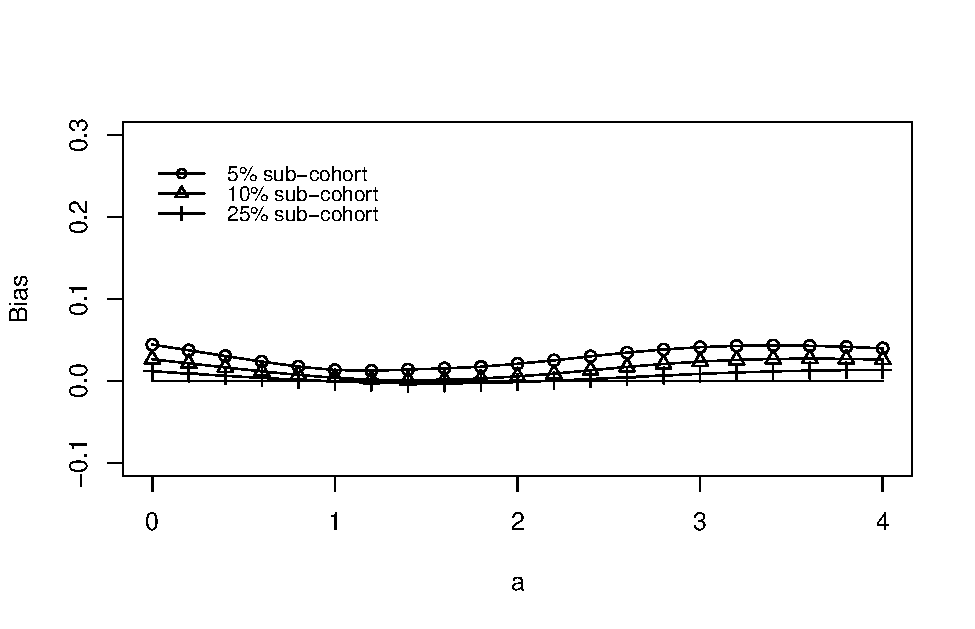
\includegraphics[width=6in]{app_fig1.pdf}
\caption{Estimated dose-response curve bias for the DR CSM method compared across three sub-cohort sizes. Bias refers to the average bias across 2,000 simulated data sets for each method evaluated at each point on the horizontal axis $a = (0, 0.2, 0.4, ..., 4)$.}
\end{figure}

\newpage

\begin{figure}
\centering
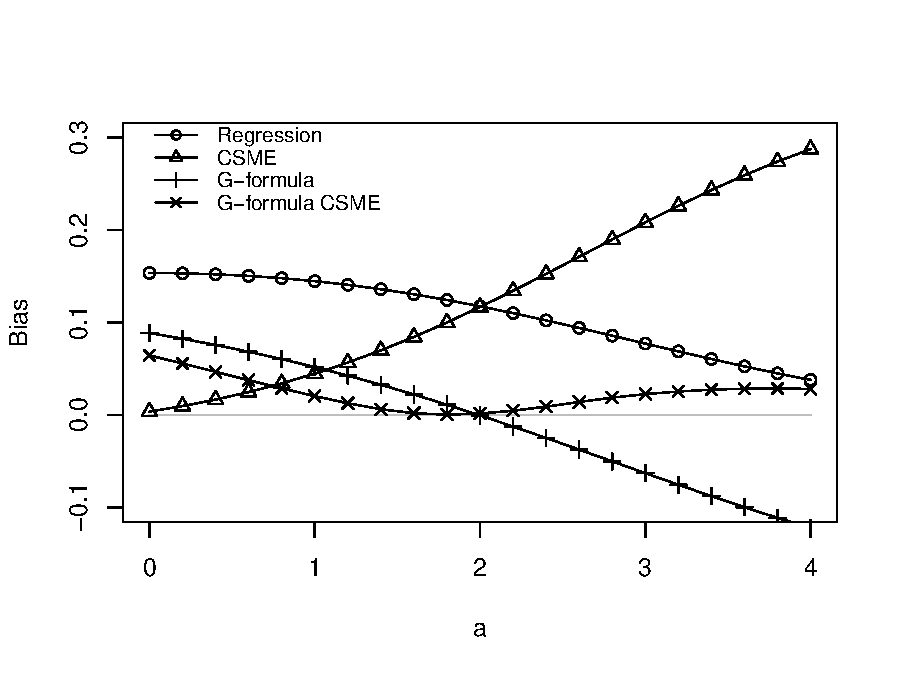
\includegraphics[width=6in]{app_fig2_updated.pdf}
\caption{Estimated dose-response curve bias for each of the four methods under positivity violation. Bias refers to the average bias across 2,000 simulated data sets for each method evaluated at each point on the horizontal axis $a = (0, 0.2, 0.4, ..., 4)$.}
\end{figure}

\clearpage
\newpage

\bibliographystyle{biom}
\bibliography{refs}

\end{document}
